\section{Auswertung}
\label{sec:auswertung}

\subsection{Mittlere Wegl"ange} % (fold)
\label{sub:mittlere_wegl_ange}


\begin{table}[!h]
\begin{center}
\begin{tabular}{|r|r|r|r|}
\hline
T[$\SI{}{^\circ}$] & $p_\mathrm{s"at}[\SI{}{\milli\bar}]$ & $\bar{w}[\SI{}{\centi\meter}]$ & $\frac{a}{\bar{w}}$\\
\hline
\hline
25  & 0.0052  & 0.5532 & 1.81\\
105 & 0.6924  & 0.0042 & 238.75\\
150 & 4.7948  & 0.0006 & 1653.38\\
190 & 19.5284 & 0.0001 & 6733.94\\
\hline
\end{tabular}
\caption[]{Errechnete Werte f"ur $p_\mathrm{s"at}$ und $\bar{w}$ in Abh"angigkeit von der Temperatur.}
\label{tab:weg}
\end{center}
\end{table}

Das Verh"altnis von der L"ange der verwendeten R"ohre $a$ zu der freien Wegl"ange der Elektronen $\bar{w}$ soll etwa einen Faktor von $1000 - 4000$ ergeben.
Nach den Formeln \eqref{eqn:p} und\eqref{eqn:w} ergaben sich die Werte aus Tabelle \ref{tab:weg} f"ur $p_\mathrm{s"at}$ und $\bar{w}$ mit $a = \SI{1}{\centi\meter}$.

Es ist zu erkennen, dass die Temperaturen $\SI{25}{^\circ}$ und $\SI{105}{^\circ}$ nicht f"ur eine Franck-Hertz Kurve geeignet sind, da das Verh"altnis zu niedrig ist.
Bei der Temperatur von $\SI{190}{^\circ}$ ist es schon etwas zu hoch, jedoch lassen sich noch akzeptable Ergebnisse erzielen, w"ahrend bei $\SI{150}{^\circ}$ das Verh"altnis in den geforderten Bereich f"allt.

\subsection{Energieverteilung der beschleunigten Elektronen} % (fold)
\label{sub:energieverteilung_der_beschleunigten_elektronen}

\subsubsection{$\si{25}{^\circ C}$} % (fold)
\label{sub:_si}


\begin{table}[!h]
\begin{center}
\begin{tabular}{|r|r|}
\hline
$U_\mathrm{a}$[V] & $\Delta y$ \\
\hline
\hline

7.000 	& 0.1 \\
7.125 	& 0.1 \\
7.250 	& 0.1 \\
7.375 	& 0.1 \\
7.500 	& 0.1 \\
7.625 	& 0.1 \\
7.750 	& 0.1 \\
7.875 	& 0.1 \\
8.000 	& 0.1 \\
8.125 	& 0.1 \\
8.250 	& 0.2 \\
8.375 	& 0.2 \\
8.500 	& 0.3 \\
8.625 	& 0.3 \\
8.750 	& 0.4 \\
8.875 	& 0.3 \\
9.000 	& 0.4 \\
9.125   & 0.4 \\
9.250 	& 0.6 \\
9.375 	& 0.8 \\
9.500 	& 1.2 \\
9.625 	& 2.0 \\
9.750 	& 3.8 \\
9.875 	& 1.5 \\

\hline
\end{tabular}
\caption[]{Wertepaare der Energieverteilung bei $\SI{25}{^\circ}$.}
\label{tab:a1}
\end{center}
\end{table}

\begin{figure}[!h]
	\centering
	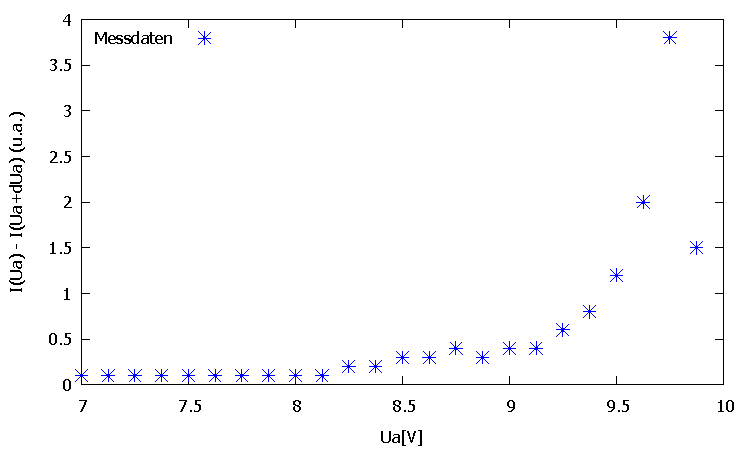
\includegraphics[width = 10cm]{img/t20.pdf}
	\caption{Energieverteilung der beschleunigten Elektronen bei $\SI{25}{^\circ}$.}
	\label{gra:25}
\end{figure}

Bei der Messung der Energieverteilung der beschleunigten Elektronen bei Zimmertemperatur ergab sich aus Tabelle \ref{a1} ein maximaler Anstieg der Kurve bei:

\begin{equation}
	U_\mathrm{a,max} = \SI{9.75}{\volt}
\end{equation}

Die Energieverteilung der Elektronen ist in Graphik \ref{gra:25} dargestellt.
Mithilfe des Zusammenhangs aus Gl. \eqref{eqn:k} ergibt sich f"ur das kontaktpotential:

\begin{equation}
	U_\mathrm{b} - U_\mathrm{b,eff} = K
\end{equation}

Mit $U_\mathrm{b} = \SI{11}{\volt}$ und $U_\mathrm{b,eff} = U_\mathrm{a,max}$ ergibt sich nun:

\begin{equation}
	K = \SI{1.25}{\volt}
\end{equation}

Qualitativ l"asst sich sagen, dass der gr"o"ste Teil der Elektronen Energien von $\SI{9.25}{\volt} - \SI{10}{\volt}$ besitzt.

\subsubsection{$\si{150}{^\circ C}$} % (fold)
\label{sub:_sis}


\begin{table}[!h]
\begin{center}
\begin{tabular}{|r|r|r|r|}
\hline
$U_\mathrm{a}$[V] & $\Delta y$ & $U_\mathrm{a}$[V] & $\Delta y$ \\
\hline
\hline

1.00 &	0.8  & 3.50 &	0.8  \\
1.25 &	0.8  & 3.75 &	0.8  \\
1.50 &	0.8  & 4.00 &	0.5  \\
1.75 &	0.8  & 4.25 &	0.4  \\
2.00 &	0.9  & 4.50 &	0.4  \\
2.25 &	0.8  & 4.75 &	0.1  \\
2.50 &	1.0  & 5.00 &	0.0  \\
2.75 &	0.8  & 5.25 &	0.0  \\
3.00 &	0.8  & 5.50 &	0.0  \\
3.25 &	0.9  & 5.75 &	0.0  \\

\hline
\end{tabular}
\caption[]{Wertepaare der Energieverteilung bei $\SI{150}{^\circ}$.}
\label{tab:a2}
\end{center}
\end{table}

\begin{figure}[!h]
	\centering
	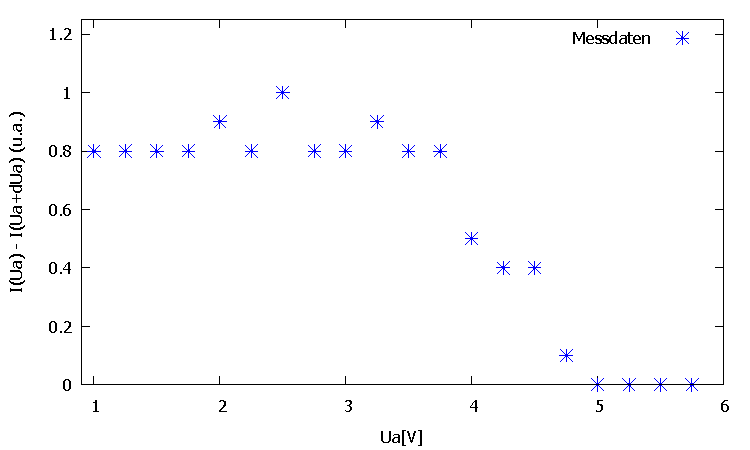
\includegraphics[width = 10cm]{img/t150.pdf}
	\caption{Energieverteilung der beschleunigten Elektronen bei $\SI{150}{^\circ}$.}
	\label{gra:150}
\end{figure}

Aus den Wertepaaren der Energieverteilung in Tabelle \ref{a2} ist zu erkennen, dass mit zunehmender Bremsspannung $U_\mathrm{a}$ sich die Energie der Elektronen dem Wert $0$ ann"ahert.
Die Werte sind in Graphik \ref{gra:150} dargestellt.

Im Vergleich zu der Kurve bei $\SI{25}{^\circ}$, welche einen Peak bei ca. $\SI{9.75}{\volt}$ besitzt, f"allt der Graph bei $\SI{150}{^\circ}$ bis ca. $\SI{4}{\volt}$ konstant.
Ab etwa $\SI{5}{\volt}$ ist die Verteilung konstant $0$.

Dieser Abbruch ist durch die Anregungsenergie der Quecksilberatome bei $U \approx \SI{4.9}{\volt}$ zu erkl"aren.
Fallen Elektronen gr"o"ser oder gleich dieser Energie auf ein Atom, gibt dieses den Anregungsbetrag an die "au"seren Elektronen ab. So dass diese Elektronen nun im niedrigen Spannungsbereich aufzufinden sind.

Der konstante Abfall der Energie l"asst sich durch die Fermie-Dirac-Verteilung erkl"aren. So nimmt die Wahrscheinlichkeit mit h"oheren Energien ab.

Die stufenartige Form der Kurve ist auf das gew"ahlte Ableseverfahren und die nahezu linearen Bereiche der integralen Kurve zurück zu f"uhren.

\subsection{Die Franck-Hertz Kurve} % (fold)
\label{sub:die_franck_hertz_kurve}


\begin{table}[!h]
\begin{center}
\begin{tabular}{|r|r|r|r|}
\hline
n-te Anregungsenergie & Anregungspotential[$\SI{}{\volt}$] & $\Delta E[\SI{1 e-19}{\electronvolt}$ & $\lambda[\SI{}{\nano\meter}]$\\
\hline
\hline
1	&	4.52	&	7.24	&	274.30\\
2	&	4.52	&	7.24	&	274.30\\
3	&	4.52	&	7.24	&	274.30\\
4	&	4.76	&	7.63	&	260.47\\
5	&	5.00	&	8.01	&	247.97\\
6	&	5.00	&	8.01	&	247.97\\
7	& 	5.24	&	8.40	&	236.61\\
\hline
\end{tabular}
\caption[]{Anregungsenergien und die daraus resultierende Anregungsenergie und die Wellenl"ange deremittierten Strahlung der Franck-Hertz Kurve.}
\label{tab:anregung}
\end{center}
\end{table}

Aus der Franck-Hertz Kurve ergaben sich die Anregungspotentiale und Energien aus Tabelle \ref{tab:anregung}. Die Anregungsenergie wurde nach Gleichung \eqref{eqn:anregung} berechnet.

F"ur die Wellenl"ange gilt:

\begin{equation}
	\lambda = \frac{h c}{e_\mathrm{0} U_\mathrm{1}}
\end{equation}

Es ist eine Abflachung und Verbreiterung der Franck-Hertz Kurve (Anhang) mit zunehmender Beschleunigungsspannung zu erkennen. Da diese jedoch nur sehr gering bei $U_\mahtrm{b} = \SI{11}{\volt}$ sind kann der Effekt der elastischen St"o"se vernachl"assigt werden.

\subsection{Ionisierungsspannung} % (fold)
\label{sub:ionisierungsspannung}

Eine Extrapolation der Kurve auf den Wert $I_\mathrm{A} = 0$ ergab:

\begin{equation}
	U_\mathrm{x} \approx \SI{13}{\volt}
\end{equation}

$U_\mathrm{ion}$ ist nun durch den Zusammenhang $U_\mathrm{ion} = U_\mathrm{x} - K$ gegeben.
Mit dem Wert f"ur K aus \ref{sub:_si} ergibt sich f"ur die Ionisationsspannung:

\begin{eqnarray*}
	U_\mathrm{ion} &\approx& \SI{11.75}{\volt} \\
\end{eqnarray*}